\documentclass[12pt]{article}

\usepackage{sbc-template}

\usepackage{graphicx,url}

\usepackage{amsmath}

\usepackage[brazil]{babel} 

\usepackage[utf8]{inputenc}  

\usepackage{placeins}
     
\usepackage{hyperref}

\usepackage[brazil]{babel}

\usepackage{graphicx}

%\usepackage[brazil]{abntex2cite}

\usepackage{listings}
\usepackage{color}

\definecolor{mygreen}{rgb}{0,0.6,0}
\definecolor{mygray}{rgb}{0.5,0.5,0.5}
\definecolor{mymauve}{rgb}{0.58,0,0.82}

\lstset{ %
  backgroundcolor=\color{white},   % choose the background color
  basicstyle=\footnotesize,        % size of fonts used for the code
  breaklines=true,                 % automatic line breaking only at whitespace
  captionpos=b,                    % sets the caption-position to bottom
  commentstyle=\color{mygreen},    % comment style
  escapeinside={\%*}{*)},          % if you want to add LaTeX within your code
  keywordstyle=\color{blue},       % keyword style
  stringstyle=\color{mymauve},     % string literal style
}

\sloppy

\title{Trabalho Prático 1\\
Kit de Ferramentas}

\author{\\Carlos Eduardo Maximo - 6962 \inst{1}\\
Pedro Emanuel de Avelar Sousa de Almeida - 6965\inst{2}\\
João Pedro Pereira da Silva - 5199\inst{3}}


\address{SIN 494 - Tópicos Especiais IV -- Universidade Federal de Viçosa (UFV)\\\\\\\\\\\\\\\\\\\\\\\\\\\\\\\\\
}

\begin{document} 

\maketitle

\section{Introdução}
O trabalho consiste em disponibilizar diversas ferramentas de verificação, conversão e cálculos numéricos, permitindo o usuário selecionar qual ferramenta deseja utilizar através de um menu.

\subsection{Ferramentas} \label{sec:arquitetura}
\begin{itemize}
\item Verifica se o número é primo;
\item Calcula a área de uma figura (funcionando para quadrado, retângulo e triângulo);
\item Calcula o enésimo elemento da sequência de Fibonacci;
\item Calcula o fatorial de um número;
\item Calcula o valor de x elevado a y (xy);
\item Calcula a média de n números inseridos;
\item Calcula máximo divisor comum entre dois números;
\item Uma calculadora com soma, subtração, multiplicação e divisão. Guardando valor uma para próxima operação;
\item Calcula a diferença entre duas datas em anos, meses e dias;
\item Converta um valor inteiro decimal para número romano;
\item Converta o tempo dado em segundos para horas, minutos e segundos;

\end{itemize}
\newpage

\section{Compilando}
\subsection {Instalação do compilador GCC em distribuições Linux}
Ubuntu e distribuições debian
\begin{itemize}
\item 1 - Abra o terminal (Ctrl + Alt + T).
\item 2 - Para verificar se o gcc está instalado em seu computador, digite no terminal gcc, caso já esteja instalado irá aparecer a seguinte mensagem “gcc : fatal error: no input files”, se não estiver instalado irá aparecer, “bash: /usr/bin/gcc: Arquivo ou diretório não encontrado”.
\item 3 - Se não existir o gcc em seu computador, rode o comando abaixo:
\begin{figure}[!htb]
     \centering
     \includegraphics[scale=0.8]{Imagens/compilando1}
     \label{Label de referência para a imagem}
\end{figure}
 
\item 4 - Após isso irá aparecer está mensagem, digite sua senha;

\begin{figure}[!htb]
     \centering
     \includegraphics[scale=0.8]{Imagens/compilando2}
     \label{Label de referência para a imagem}
\end{figure}

\item 5 - Feito isso a instalação será executada, espere até que finalize.

\begin{figure}[!htb]
     \centering
     \includegraphics[scale=0.8]{Imagens/compilando3}
     \label{Label de referência para a imagem}
\end{figure}

\item 6 - Pronto gcc instalado.

\end{itemize}

\newpage

\subsection {Instalação da IDE (Visual Studio Code, Sublime Text, Code Blocks, NetBeans)}
Existem várias IDE’s para programar em C, neste manual iremos ensinar a instalar o Vscode, mas fique a vontade para escolher outro.
\begin{itemize}
\item 1 - Abra o navegador e digite vscode, https://code.visualstudio.com/
\item 2 - Depois clique em Download, irá baixar o executável em seu computador.
\item 3 - Finalizado o Download, abra o arquivo.
\item 4 - Clique para instalar.
\item 5 - Programa instalado, abra e vá:

\begin{figure}[!htb]
     \centering
     \includegraphics[scale=0.8]{Imagens/compilando4}
     \label{Label de referência para a imagem}
\end{figure}

\item 6 - Após ter clicado no ícone de extensões digite C.

\begin{figure}[!htb]
     \centering
     \includegraphics[scale=0.8]{Imagens/compilando5}
     \label{Label de referência para a imagem}
\end{figure}

\item 7 - Clique em instalar.
 
\item 8 - Pronto agora você pode rodar qualquer programa com a extensão arquivo.c, para compilar os programas, é necessário rodar o comando gcc arquivo.c -o arquivo \&\& ./arquivo .

\end{itemize}

\newpage

\section{Menu} \label{sec:analise}
Ao acessar o programa, a primeira coisa que é exibida para o usuário é o menu de seleção, onde permite o usuário digitar o número da ferramente para acessá-la, por exemplo, se o usuário digitar o dígito 4, irá para a ferramente 'Calcular o Fatorial de um numero'. \\
Assim que o usuário utilizar a ferramenta, o programa não irá encerrar, será exibido o menu novamente para poder selecionar uma outra funcionalidade do programa. Para encerrar, é necessário digitar o dígito 12.\\

\begin{figure}[!htb]
     \centering
     \includegraphics[scale=1]{Imagens/menu}
     \caption{Menu do Programa}
     \label{Label de referência para a imagem}
\end{figure}

\newpage

\section{Verificar se o número é primo}
Permite ao usuário digitar qualquer valor inteiro para o programa analisar se o valor digitado é primo ou não, isto é, se o número é dividido apenas por um e por ele mesmo. \\
O código consiste em ter uma variável 'cont' que inicia em 1, e é incrementado de 1 em 1, enquanto isso é verificado se o número digitado pelo usuário é divisível por esta variável 'cont', ao final, é verificado quantas vezes o número do usuário foi divisível pelo 'cont' para verificar se é primo ou não, como é possível analisar pela imagem a seguir:

\begin{figure}[!htb]
     \centering
     \includegraphics[scale=1]{Imagens/primo}
     \caption{Código da Ferramenta 1}
     \label{Label de referência para a imagem}
\end{figure}

A seguir é possível analisar alguns exemplos inseridos no programa e o retorno que foi obtido:

\FloatBarrier
\begin{table}[ht]
\centering
\begin{tabular}{|l|l|}
\hline
\textbf{Entrada} & \textbf{Saida}\\
\hline
7 & O valor digitado e primo\\
12 & O valor digitado nao e primo\\
332 & O valor digitado nao e primo\\
487 & O valor digitado e primo\\
991 & O valor digitado e primo\\
993 & O valor digitado nao e primo\\

\hline
\end{tabular}
\caption{Entradas e Saídas da Ferramenta 1}
\end{table} 

\newpage

\section{Calcula área de uma figura}
Ao selecionar esta opção, irá abrir um novo menu para selecionar qual figura irá ter sua área calculada. Dependendo da área selecionada, o programa irá solicitar a informação de acordo, por exemplo, ao selecionar a Área do Quadrado, o programa irá solicitar somente o Lado, enquanto a Área do Triangulo será solicitado a Base e a Altura. O número de entrada digitado pelo usuário pode conter número decimal, e a saída exibe 2 casas decimais.

\subsection{Áreas permitidas}
\begin{itemize}
\item Calcular Área do Triângulo;
\subitem Cálculo: (base * altura ) / 2;
\item Calcular Área do Quadrado;
\subitem Cálculo: lado * lado;
\item Calcular Área do Retângulo;
\subitem Cálculo: base * altura;
\end{itemize}
A seguir é possível analisar alguns exemplos inseridos no programa e o retorno que foi obtido:

\FloatBarrier
\begin{table}[ht]
\centering
\begin{tabular}{|l|c|l|}
\hline
\textbf{Área} & \textbf{Entrada} & \textbf{Saida}\\
\hline
Triângulo & 4 - 5 & A area do Triangulo calculado e: 10.00\\
Triângulo & 12.78 - 17.11 & A area do Triangulo calculado e: 109.33\\
Quadrado & 23 & A area do Quadrado calculado e: 529.00\\
Quadrado & 41.93 & A area do Quadrado calculado e: 1758.12\\
Retângulo & 6 - 2 & A area do Retângulo calculado e: 12.00\\
Retângulo & 38.92 - 31.06 & A area do Retângulo calculado e: 1208.86\\

\hline
\end{tabular}
\caption{Entradas e Saídas da Ferramenta 2}
\end{table} 

\newpage

\section{Calcula o enésimo elemento da sequência de Fibonacci}
Esta ferramente permite ao usuário digitar um número inteiro positivo que corresponde a posição que ele deseja buscar da sequência de Fibonacci, que é uma sequência de números inteiros, começando por 0 e 1, na qual, cada termo subsequente corresponde à soma dos dois anteriores. \\
A seguir uma parte da sequência de Fibonacci:\\
0, 1, 1, 2, 3, 5, 8, 13, 21, 34, 55, 89, 144, 233, 377, 610, 987, 1597, ...
Em código, foi utilizado 3 variáveis para armazenar os dados, onde uma guarda a soma dos dois anteriores, enquanto as outras duas variáveis armazena os próprios valores anteriores, como é possível analisar pela imagem a seguir:

\begin{figure}[!htb]
     \centering
     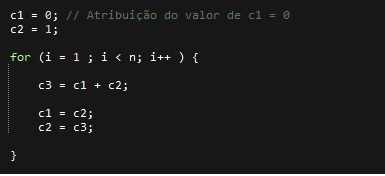
\includegraphics[scale=1]{Imagens/Fibonacci}
     \caption{Código da Ferramenta 3}
     \label{Label de referência para a imagem}
\end{figure}

A seguir é possível analisar alguns exemplos inseridos no programa e o retorno que foi obtido:

\FloatBarrier
\begin{table}[ht]
\centering
\begin{tabular}{|l|l|}
\hline
\textbf{Entrada} & \textbf{Saida}\\
\hline
7 & O 7 elemento e: 8\\
13 & O 13 elemento e: 144\\
2 & O 2 elemento e: 1\\
16 & O 16 elemento e: 610\\

\hline
\end{tabular}
\caption{Entradas e Saídas da Ferramenta 3}
\end{table} 

\newpage

\section{Calcula o fatorial de um número}
Permite ao usuário digitar um numero inteiro positivo para calcular o seu fatorial.
O fatorial de um número é calculado pela multiplicação desse número por todos os seus antecessores até chegar ao número 1.
O fatorial é representado por: n! = n . (n – 1) . (n – 2) . (n – 3)...
O código foi feito com uma estrutura de repetição que inicia igual ao número digitado pelo usuário que é decrementado até chegar a 1, enquanto isso é guardado na variável 'c1' o valor de 'c1' multiplicado pelo número do controle da estrutura de repetição, como é possível analisar pela imagem a seguir:

\begin{figure}[!htb]
     \centering
     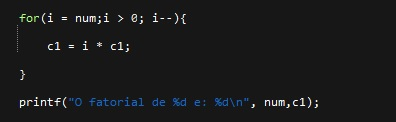
\includegraphics[scale=1]{Imagens/Fatorial}
     \caption{Código da Ferramenta 4}
     \label{Label de referência para a imagem}
\end{figure}

A seguir é possível analisar alguns exemplos inseridos no programa e o retorno que foi obtido:

\FloatBarrier
\begin{table}[ht]
\centering
\begin{tabular}{|l|l|}
\hline
\textbf{Entrada} & \textbf{Saida}\\
\hline
2 & O fatorial e: 2\\
9 & O fatorial e: 362880\\
5 & O fatorial e: 120\\
7 & O fatorial e: 5040\\

\hline
\end{tabular}
\caption{Entradas e Saídas da Ferramenta 4}
\end{table} 

\newpage

\section{Calcula o valor de x elevado a y (xy)}
Ao selecionar esta opção, irá pedir ao usuário para inserir o valor de x (base) e o valor de y (expoente), podendo assim o programa multiplar a base x por ela mesma quantas vezes indicar o expoente y, a seguir, a parte do código relacionado a este cálculo:

\begin{figure}[!htb]
     \centering
     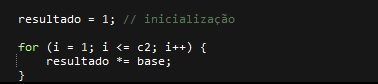
\includegraphics[scale=1]{Imagens/Exponenciacao}
     \caption{Código da Ferramenta 5}
     \label{Label de referência para a imagem}
\end{figure}

A seguir é possível analisar alguns exemplos inseridos no programa e o retorno que foi obtido:

\FloatBarrier
\begin{table}[ht]
\centering
\begin{tabular}{|l|l|l|}
\hline
\textbf{Entrada X} & \textbf{Entrada Y} & \textbf{Saida}\\
\hline
3 & 2 & O resultado de 3.00 elevado a 2 e: 6.00\\
6 & 7 & O resultado de 6.00 elevado a 7 e: 279936.00\\
5.21 & 3 & O resultado de 5.21 elevado a 3 e: 141.42\\
1 & 0 & O resultado de 1.00 elevado a 0 e: 1.00\\

\hline
\end{tabular}
\caption{Entradas e Saídas da Ferramenta 5}
\end{table} 

\newpage

\section{Calcula a média de n números inseridos}
Assim que selecionar esta ferramenta, irá solicitar ao usuário diversos números para calcular a média, o programa só irá efetuar o cálculo assim que o usuário informar o dígito de encerramento, que é o número 0. \\
A média é a soma de todos os números divido pela quantidade de números informados, a seguir é possível analisar a parte do código relacionado a este cálculo:

\begin{figure}[!htb]
     \centering
     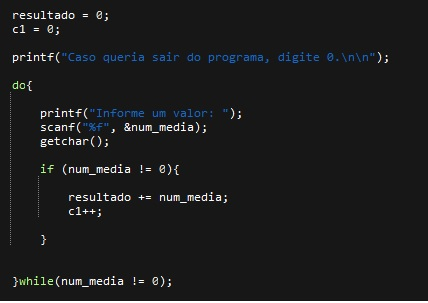
\includegraphics[scale=1]{Imagens/Media}
     \caption{Código da Ferramenta 6}
     \label{Label de referência para a imagem}
\end{figure}

A seguir é possível analisar alguns exemplos inseridos no programa e o retorno que foi obtido:

\FloatBarrier
\begin{table}[ht]
\centering
\begin{tabular}{|l|l|}
\hline
\textbf{Entrada} & \textbf{Saida}\\
\hline
2;  7;  8;  2 & 4.75\\
6;  9;  2;  1; 34 & 52.00\\
9;  4 & 6.50\\
41; 7;  23 & 23.67\\

\hline
\end{tabular}
\caption{Entradas e Saídas da Ferramenta 6}
\end{table} 

\newpage

\section{Cálcula o máximo divisor comum entre dois números}
Ao selecionar esta opção, é solicitado ao usuário informar dois números inteiros, dessa forma o programa irá calcular o MDC dos dois números. \\
O MDC (máximo divisor comum) é o maior número possível divisível que possui resto igual a 0. \\
O programa consiste em verificar cada número inferior aos números informados para analisar se são divisíveis através de duas estruturas de repetição em cadeia, ao final, informa ao usuário o resultado. \\
A seguir é possível analisar alguns exemplos inseridos no programa e o retorno que foi obtido:

\FloatBarrier
\begin{table}[ht]
\centering
\begin{tabular}{|l|l|l|}
\hline
\textbf{Entrada 1} & \textbf{Entrada 2} & \textbf{Saida}\\
\hline
44 & 11 & O MDC dos numeros digitados e: 11\\
462 & 102 & O MDC dos numeros digitados e: 6\\
57 & 1932 & O MDC dos numeros digitados e: 3\\
250 & 750 & O MDC dos numeros digitados e: 250\\

\hline
\end{tabular}
\caption{Entradas e Saídas da Ferramenta 7}
\end{table} 

\newpage

\section{Uma calculadora com soma, subtração, multiplicação e divisão. Guardando valor para uma para próxima operação}
Ao selecionar esta opção, é exibido um menu com as opções de cálculo disponível, o usuário deverá digitar o símbolo para efetuar o cálculo desejado. \\
Opções disponíveis:
\begin{itemize}
\item Soma [+]
\item Subtracao [-]
\item Divisao [/]
\item Multiplicacao [*]
\item Sair [E]
\end{itemize}
Depois que efetuar o cálculo, é retornado para o menu para o usuário poder efetuar novamente outro cálculo juntamente com o resultado anterior. \\
A seguir é possível analisar alguns exemplos inseridos no programa e o retorno que foi obtido:

\FloatBarrier
\begin{table}[ht]
\centering
\begin{tabular}{|l|l|l|l|}
\hline
\textbf{Operador} & \textbf{Entrada 1} & \textbf{Entrada 2} & \textbf{Saida}\\
\hline
+ & 10 & 10 & A soma de 10.00 e 10.00 e: 20.00 \\
- & 8 & 3 & A subtracao de 5.00 e 20.00 e: 15.00 \\
/ & 5.21 & 3.47 & A divisao de 15.00 por 1.50 e: 9.99 \\
* & 7 & 54.86 & A multiplicacao de 9.99 por 384.02 e: 3836.51 \\

\hline
\end{tabular}
\caption{Entradas e Saídas da Ferramenta 8}
\end{table} 

\newpage

\section{Calcula a diferença entre duas datas em anos, meses e dias}
Está ferramente pede ao usuário digitar o dia, mês e ano separadamente das duas datas que serão comparadas, e ao final do programa, é exibido a diferença em dias, meses e anos. \\
É possível analisar a saída do programa na imagem a seguir:

\begin{figure}[!htb]
     \centering
     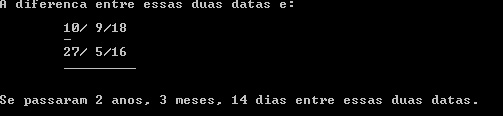
\includegraphics[scale=1]{Imagens/Data}
     \caption{Código da Ferramenta 9}
     \label{Label de referência para a imagem}
\end{figure}

A seguir é possível analisar alguns exemplos inseridos no programa e o retorno que foi obtido:

\FloatBarrier
\begin{table}[ht]
\centering
\begin{tabular}{|l|l|l|}
\hline
\textbf{Entrada 1} & \textbf{Entrada 2} & \textbf{Saida}\\
\hline
27/3/2019 & 23/1/2019 & Se passaram 0 anos, 2 meses, 4 dias entre essas duas datas\\
4/1/2001 & 4/1/2001 & Se passaram 0 anos, 0 meses, 0 dias entre essas duas datas\\
23/6/2015 & 5/1/2011 & Se passaram 4 anos, 5 meses, 18 dias entre essas duas datas\\
10/10/2010 & 20/12/2020 & Se passaram 10 anos, 2 meses, 10 dias entre essas duas datas\\

\hline
\end{tabular}
\caption{Entradas e Saídas da Ferramenta 9}
\end{table} 

\newpage

\section{Converta um valor inteiro decimal para número romano}
Os números romanos foram durante muito tempo a principal forma de representação numérica na Europa. Os números eram representados a partir de letras do próprio alfabeto dos romanos. Esse sistema numérico associava uma letra a uma quantidade fixa.\\
A ferramenta 10 permite converter um valor decimal para números romanos, de acorda com a tabela a seguir:

\begin{figure}[!htb]
     \centering
     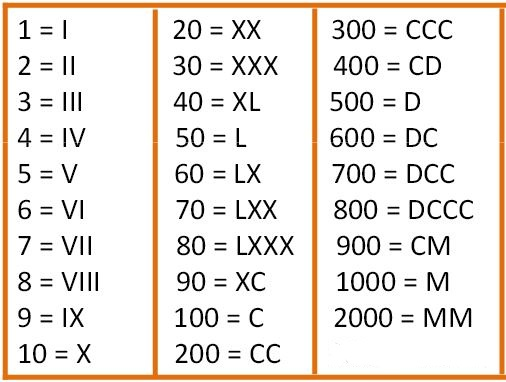
\includegraphics[scale=1]{Imagens/tabelaRomanos}
     \caption{Tabela de números romanos}
     \label{Label de referência para a imagem}
\end{figure}

A seguir é possível analisar alguns exemplos inseridos no programa e o retorno que foi obtido:

\FloatBarrier
\begin{table}[ht]
\centering
\begin{tabular}{|l|l|}
\hline
\textbf{Entrada} & \textbf{Saida}\\
\hline
405 &  O numero 405 em romano e: CDV\\
1823 &  O numero 1823 em romano e: MDCCCXXIII\\
29 &  O numero 29 em romano e: XXIX\\
7 &  O numero 7 em romano e: VII\\

\hline
\end{tabular}
\caption{Entradas e Saídas da Ferramenta 10}
\end{table} 

\newpage

\section{Converta o tempo dado em segundos para horas, minutos e segundos}
Esta ferramenta foi a escolhida pelo grupo, consiste em solicitar um tempo em segundos ao usuário para converter no formato de hora usual (horas, minutos e segundos).\\
O programa efetua cálculos de divisão juntamente com mod para conseguir chegar ao resultado correto, a seguir possui a parte do código relacionado a este cálculo:
\begin{figure}[!htb]
     \centering
     \includegraphics[scale=1]{Imagens/segundos}
     \caption{Código da Ferramenta 11}
     \label{Label de referência para a imagem}
\end{figure}

A seguir é possível analisar alguns exemplos inseridos no programa e o retorno que foi obtido:

\FloatBarrier
\begin{table}[ht]
\centering
\begin{tabular}{|l|l|}
\hline
\textbf{Entrada} & \textbf{Saida}\\
\hline
20345 &  5 horas, 39 minutos e 5 segundos\\
294 &  0 horas, 4 minutos e 54 segundos\\
92847 &  25 horas, 47 minutos e 27 segundos\\
34 &  0 horas, 0 minutos e 34 segundos\\

\hline
\end{tabular}
\caption{Entradas e Saídas da Ferramenta 11}
\end{table} 

\end{document}